\documentclass[10pt,pdf,hyperref={unicode}]{beamer} %aspectratio=169-для 16:9
\usepackage[T2A]{fontenc}
\usepackage[utf8]{inputenc}
\usepackage[english,russian]{babel} 
\usepackage{amssymb,amsfonts,amsmath,mathtext}
\usepackage{cite,enumerate,float,indentfirst}
\usepackage{graphicx}
\usepackage{multimedia}
\usepackage{hyperref}
\usepackage{pgfplots}
\usepackage{pgfplotstable}
\usepackage{subfig}

%%%%%%%%%%%
\usepackage{tikz}
\usetikzlibrary{shapes,arrows}

\tikzstyle{startstop} = [rectangle, rounded corners, minimum width=1.5cm, minimum height=1.5cm, text centered, draw=black, fill=red!20]
\tikzstyle{io} = [trapezium, trapezium left angle=70, trapezium right angle=110, minimum width=2cm, minimum height=1cm, text centered, text width=2cm, draw=black, fill=orange!20]
\tikzstyle{io2} = [trapezium, trapezium left angle=70, trapezium right angle=110, minimum width=3cm, minimum height=1cm, text centered, text width=3cm, draw=black, fill=orange!20]
\tikzstyle{process} = [rectangle, minimum width=2cm, minimum height=1cm, text centered, text width=2cm, draw=black, fill=blue!20]
\tikzstyle{process2} = [rectangle, minimum width=3cm, minimum height=1cm, text centered, text width=3cm, draw=black, fill=blue!20]
\tikzstyle{decision} = [diamond, minimum width=1cm, minimum height=1cm, text centered, draw=black, fill=green!20]
\tikzstyle{arrow} = [thick, ->, >=stealth]

%%%%%%%%%%%%

\renewcommand{\rmdefault}{ftm}

\addto\captionsrussian{%
\renewcommand{\figurename}{}%
\renewcommand{\tablename}{}%
}

\graphicspath{{fig/}}

\usetheme{Boadilla}
\usecolortheme{crane}
%\usefonttheme[onlylarge]{structurebold}
\usefonttheme[onlymath]{serif}
\setbeamerfont{institute}{size=\normalsize}
\setbeamercolor{color1}{bg=blue!60!black,fg=white}
\beamertemplatenavigationsymbolsempty

\makeatletter
\defbeamertemplate*{footline}{my theme}{
    \leavevmode
    \hbox{
    \begin{beamercolorbox}[wd=\paperwidth,ht=2.25ex,dp=1ex,right]{date in head/foot}
        \insertframenumber{} / \inserttotalframenumber \hspace*{2ex}
    \end{beamercolorbox}}
}
\makeatother

\title{ Решение задач трехфазной неизотермической фильтрации \\
на высокопроизводительных вычислительных системах}
\author{Люпа Анастасия Александровна}
\institute{Московский физико-технический институт \\
(государственный университет)\\
%\vspace{0.1cm}
Факультет управления и прикладной математики \\
Кафедра математического моделирования \\
    \vspace{0.2cm}
    Научный руководитель: с.н.с., к.ф.-м.н. Чурбанова Н.Г.\\
}
\date{
    Москва 2014г.
}

\begin{document}

\begin{frame}
  \maketitle
\end{frame}

\section{Содержание}

\begin{frame}
\begin{center}
\frametitle{Содержание}
\framesubtitle{\ }
\begin{itemize}
\item {\large Введение}
\vspace{0.3cm}
\item {\large Цели работы}
\vspace{0.3cm}
\item {\large Математическая модель трехфазной фильтрации}
\vspace{0.3cm}
\item {\large Алгоритм расчета модели}
\vspace{0.3cm}
\item {\large Параллельная реализация алгоритма}
\vspace{0.3cm}
\item {\large Тестовые задачи}
\vspace{0.3cm}
\item {\large Анализ производительности системы}
\vspace{0.3cm}
\item {\large Заключение}
\end{itemize}
\end{center}
\end{frame}

\section{Введение}

\begin{frame}
\begin{center}
\frametitle{Введение}
\framesubtitle{\ }
\begin{figure}
\begin{minipage}[h]{0.43\textwidth}
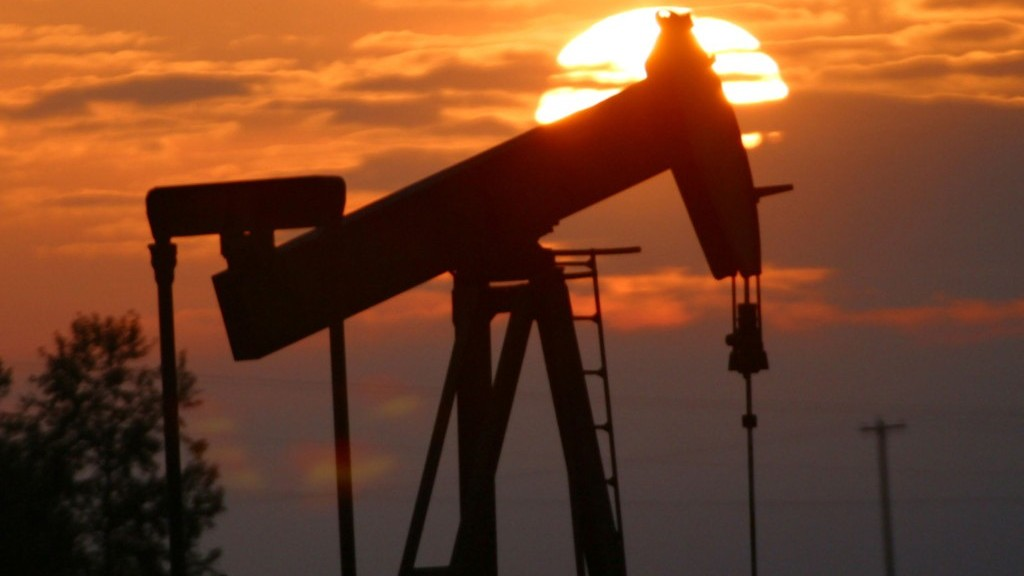
\includegraphics[width=1.0\textwidth]{oil_pump169.jpg}
\caption{\small{Добыча нефти и газа\\ \ }}
\end{minipage}
\hspace{8mm}
\begin{minipage}[h]{0.43\textwidth}
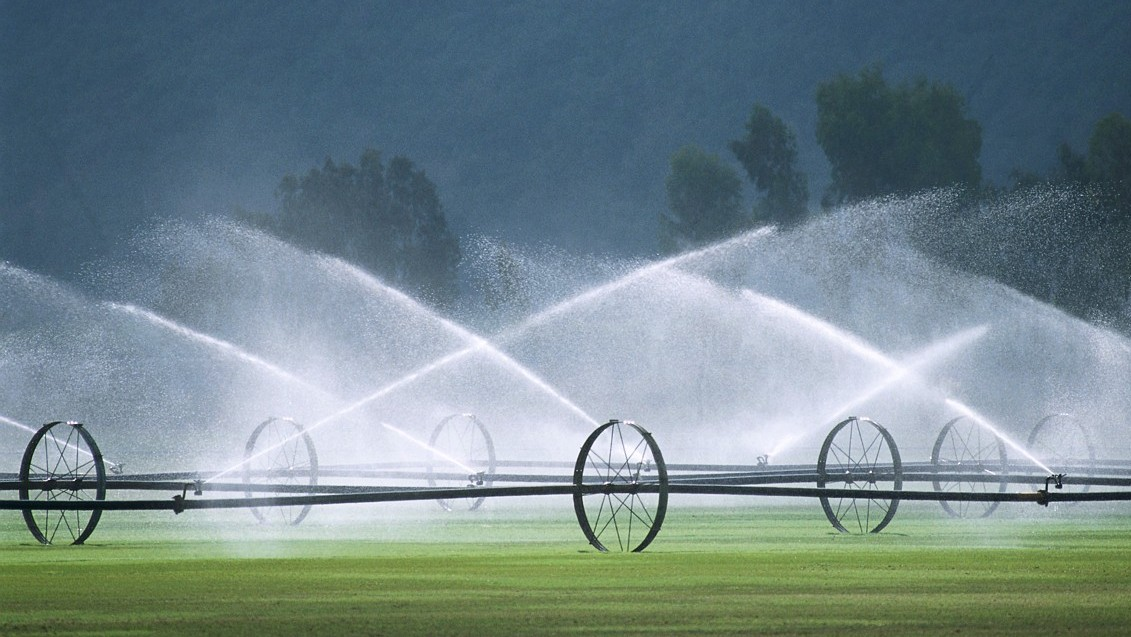
\includegraphics[width=1.0\textwidth]{melio169.jpg}
\caption{\small{Мелиоративные сооружения\\ \ }}
\end{minipage}
\vfill
\begin{minipage}[h]{0.43\textwidth}
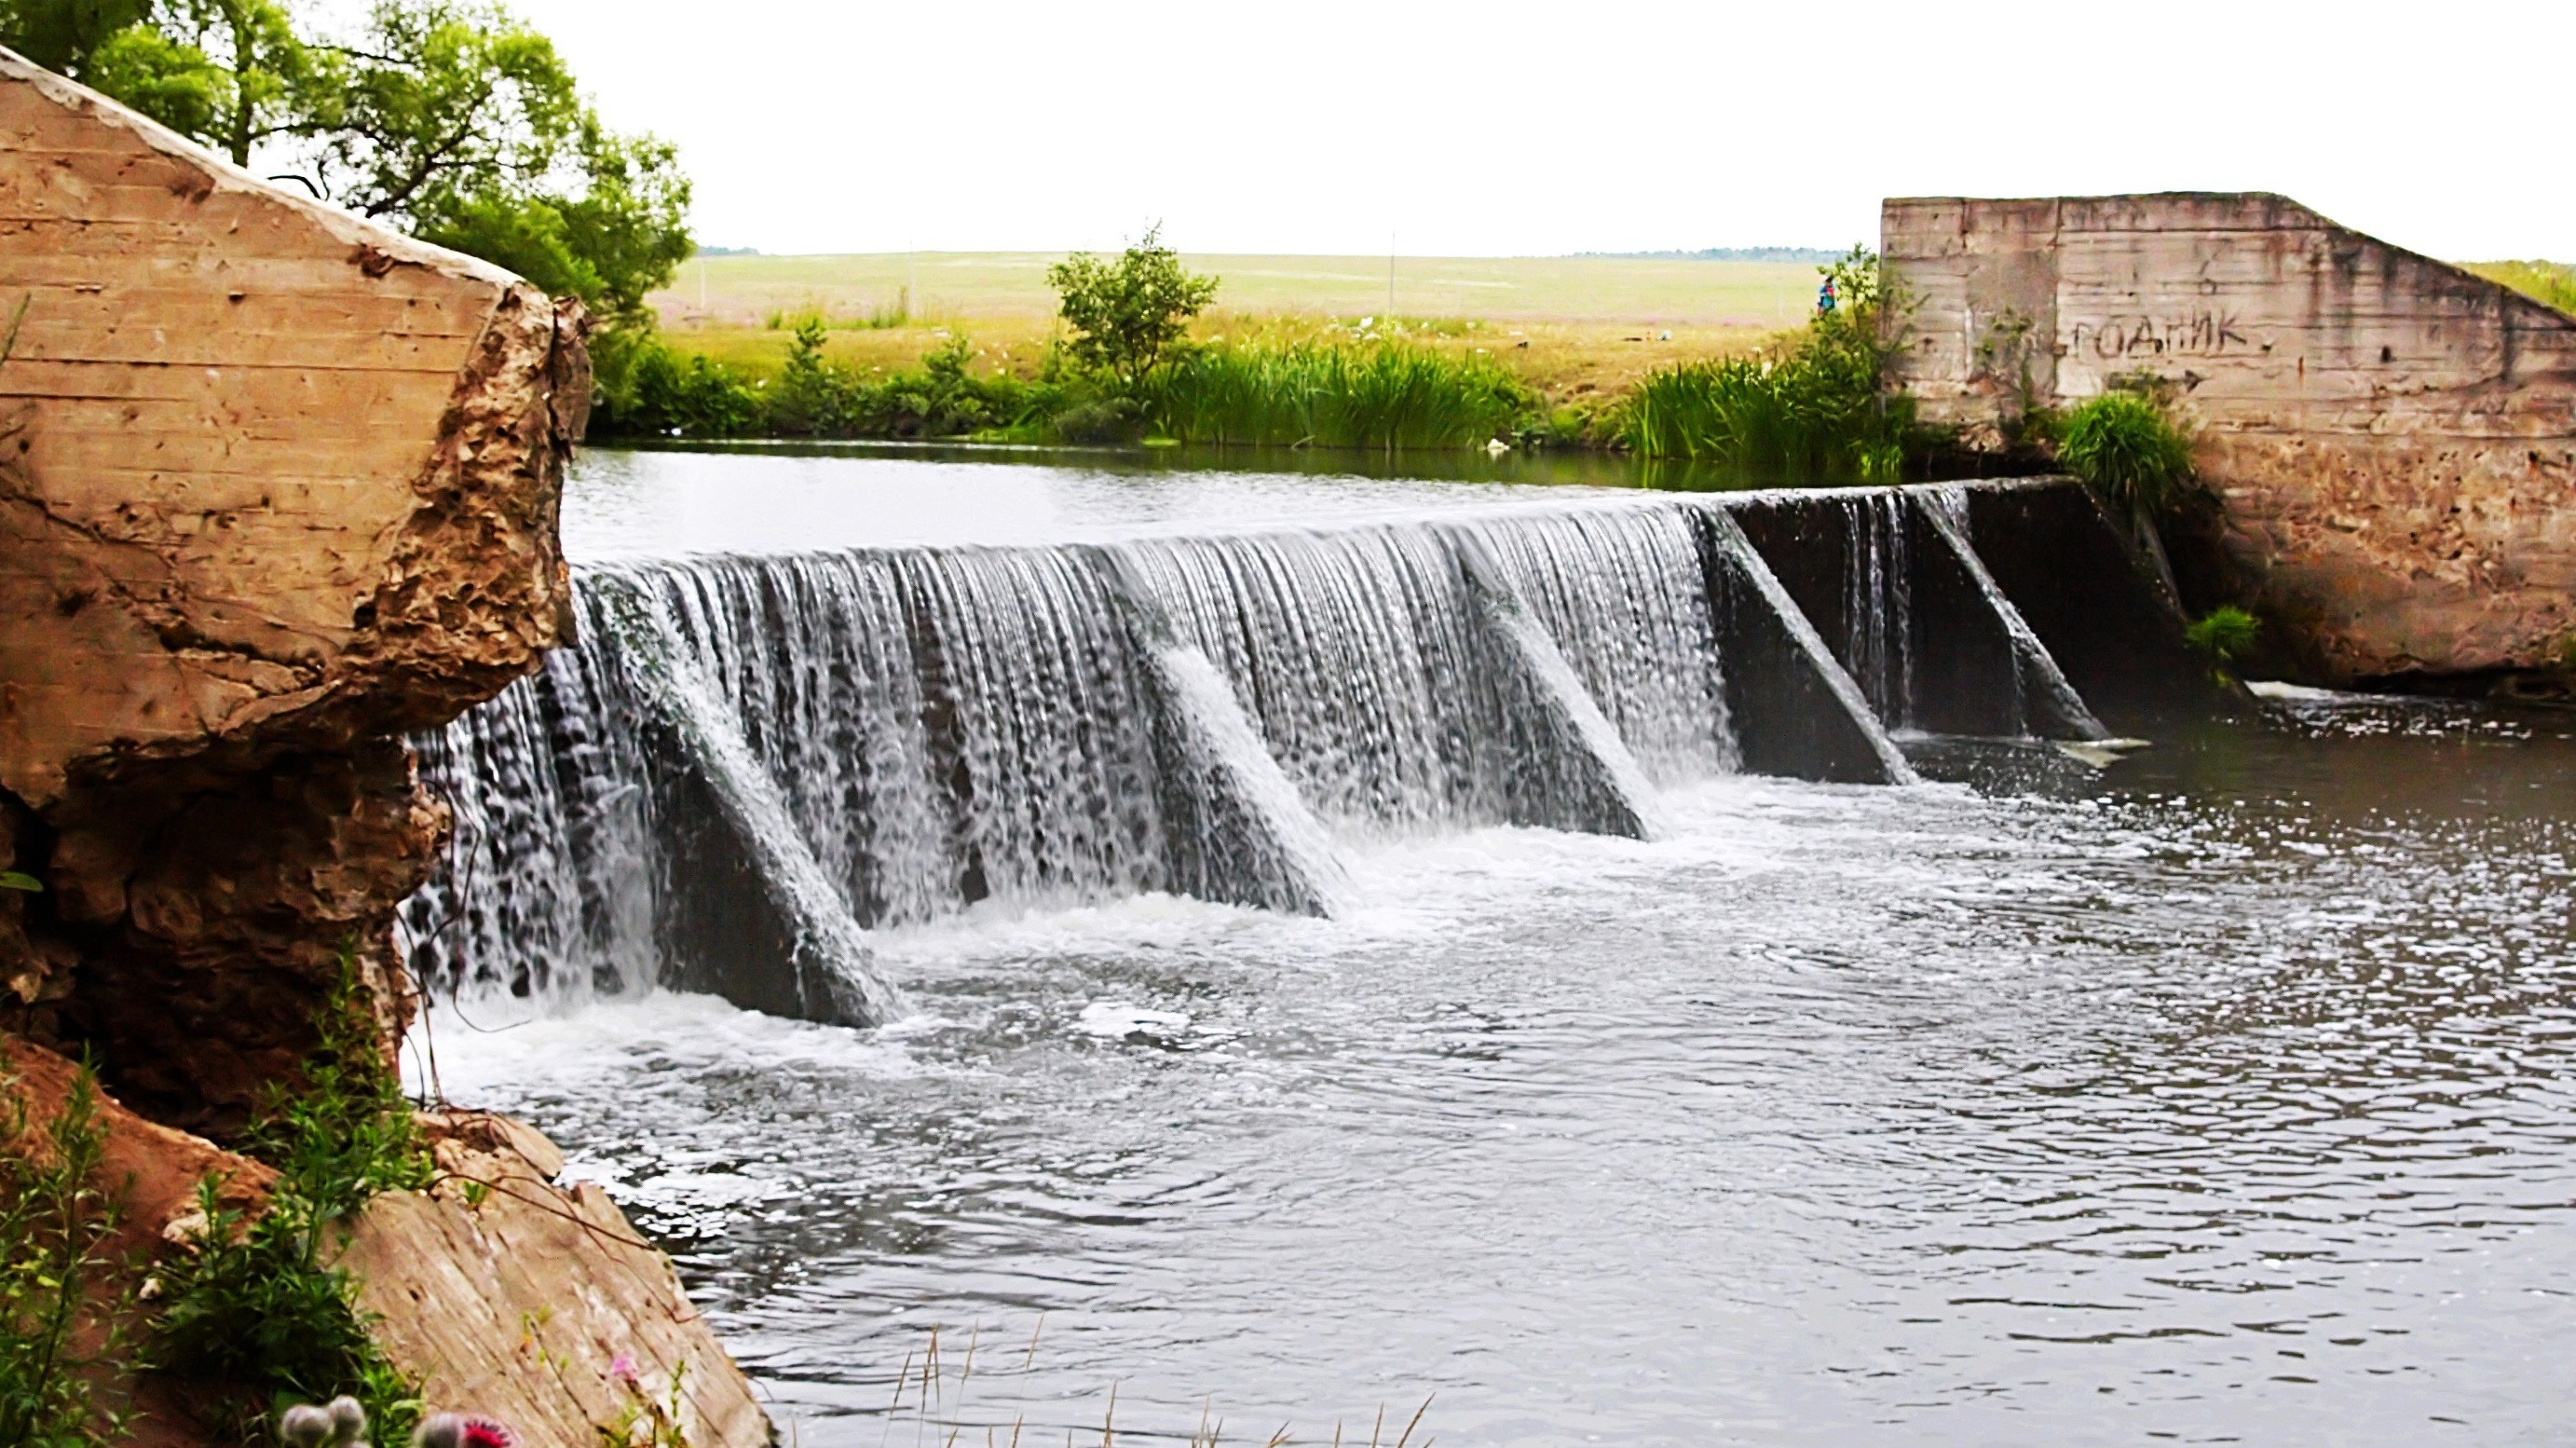
\includegraphics[width=1.0\textwidth]{plotina169.jpg}
\caption{\small{Гидротехнические сооружения}}
\end{minipage}
\hspace{8mm}
\begin{minipage}[h]{0.43\textwidth}
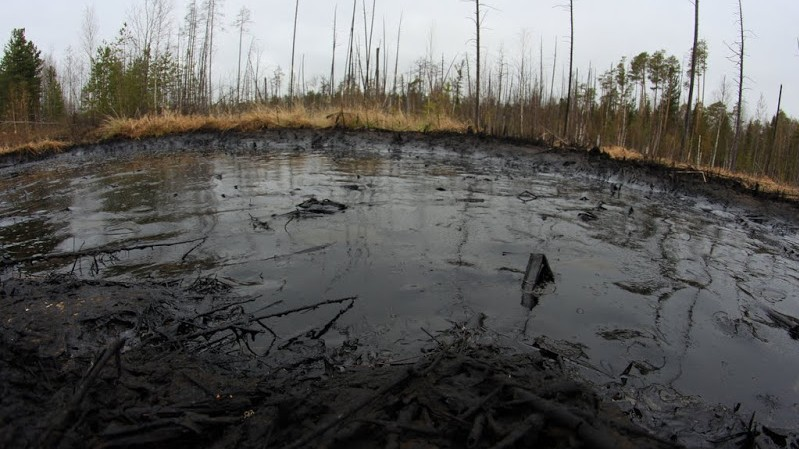
\includegraphics[width=1.0\textwidth]{dirty169.jpg}
\caption{\small{Решение экологических проблем}}
\end{minipage}
\end{figure}
\end{center}
\end{frame}

\section{Цели работы}

\tikzstyle{itembox} = [rectangle, rounded corners, minimum width=1.5cm, minimum height=1.5cm, text centered, draw=black, fill=GreenYellow!50]

\begin{frame}
\begin{center}
\frametitle{Цели работы}
\framesubtitle{\ }
\begin{figure}
  \begin{minipage}[h]{0.2\textwidth}
    
\includegraphics[width=1.0\textwidth]{aim.png}
  \end{minipage}
  \hspace{-1cm}
  \begin{minipage}[h]{0.75\textwidth}
    \begin{tikzpicture}[]
      \node (item1) [itembox, xshift=5.0cm] {Математическая модель};
      \node (item2) [itembox, right of=item1, xshift=4.5cm, yshift=-0.5cm]{Явные численные методы};
      \node (item3) [itembox, below of=item1, xshift=2.0cm, yshift=-1.0cm] {Алгоритм};
      \node (item4) [itembox, below of=item2, yshift=-1.0cm] {Программа};
      \node (item5) [itembox, below of=item3, yshift=-1.0cm] {Многопроцессорные системы};
      \node (item6) [itembox, left of=item5, xshift=-1.0cm, yshift=-2.0cm] {Графические ускорители};
      \node (item7) [itembox, below of=item5, xshift=3.0cm, yshift=-1.0cm] {Тестовые задачи};
    \end{tikzpicture}
  \end{minipage}
\end{figure}
\end{center}
\end{frame}

\section{Математическая модель трехфазной фильтрации}

\begin{frame}
\begin{center}
\frametitle{Математическая модель трехфазной фильтрации}
\framesubtitle{Основные предположения}
\begin{itemize}
\item Трехфазные течения: вода, легкая нефть и газ
\vspace{0.3cm}
\item Фазы несмешивающиеся
\vspace{0.3cm}
\item Жидкости слабосжимаемые
\vspace{0.3cm}
\item Газ идеальный
\vspace{0.3cm}
\item Среда пористая, однородная, изотропная, неподвижная
\vspace{0.3cm}
\item Учитываются капиллярные силы и гравитационное поле
\vspace{0.3cm}
\item Учитываются тепловые процессы
\end{itemize}
\end{center}
\end{frame}

\begin{frame}
\begin{center}
\frametitle{Математическая модель трехфазной фильтрации}
\framesubtitle{Полная система уравнений}
\begin{equation*}
\left\{
  \begin{aligned}
    & \text{1)}\ \frac{\partial \left(m {\sum\limits_{i}{\rho_i S_i E_i(P_i, T)}} + (1-m){\rho_r E_r(P_w, T)}\right)}{\partial t} + \\
    & \qquad + div(\sum_{i}{\rho_i H_i(T) \overrightarrow{u_i}}) = div(\lambda_{eff} grad T),\\
    & \text{2)}\ \frac{\partial (m \rho_i S_i)}{\partial t}+ div(\rho_i \overrightarrow{u_i}) = \rho_i q_i,\\
    & \text{3)}\ \overrightarrow{u_i}=-K \frac{k_i}{{\mu_i(T)}}(grad P_i - {\rho}_i\overrightarrow{g}),\\
    & \text{4)}\ S_w + S_n + S_g=1,\\
    & \text{5)}\ P_n=P_w+P_{cnw}(\overline{S_w}),\quad P_g=P_w+P_{cnw}(\overline{S_w})+P_{cgn}(\overline{S_g}),\\
    & \text{6)}\ k_w=k_w(\overline{S_w}),\quad k_g=k_g(\overline{S_g}),\quad k_n=k_n(\overline{S_w},\overline{S_n}),\\
    & \text{7)}\ \rho_i=\rho_i(P_i,T),\\
    &i=w,n,g. \\
  \end{aligned}
\right.
\end{equation*}
\end{center}
\end{frame}

\begin{frame}
\begin{center}
\frametitle{Математическая модель трехфазной фильтрации}
\framesubtitle{Полная система уравнений с модифицированным уравнением неразрывности}
\begin{equation*}
\left\{
  \begin{aligned}
    & \text{1)}\ \frac{\partial \left(m {\sum\limits_{i}{\rho_i S_i E_i(P_i, T)}} + (1-m){\rho_r E_r(P_w, T)}\right)}{\partial t} + \\
    & \qquad + div(\sum_{i}{\rho_i H_i(T) \overrightarrow{u_i}}) = div(\lambda_{eff} grad T),\\
    & \text{2)}\ \frac{\partial (m \rho_i S_i)}{\partial t}+ div(\rho_i \overrightarrow{u_i}) = \rho_i q_i\textcolor{red}{ + l c_i \cdot div(grad(\rho_i S_i))}, \\
    & \text{3)}\ \overrightarrow{u_i}=-K \frac{k_i}{{\mu_i(T)}}(grad P_i - {\rho}_i\overrightarrow{g}),\\
    & \text{4)}\ S_w + S_n + S_g=1,\\
    & \text{5)}\ P_n=P_w+P_{cnw}(\overline{S_w}),\quad P_g=P_w+P_{cnw}(\overline{S_w})+P_{cgn}(\overline{S_g}),\\
    & \text{6)}\ k_w=k_w(\overline{S_w}),\quad k_g=k_g(\overline{S_g}),\quad k_n=k_n(\overline{S_w},\overline{S_n}),\\
    & \text{7)}\ \rho_i=\rho_i(P_i,T),\\
    &i=w,n,g. \\
  \end{aligned}
\right.
\end{equation*}
\end{center}
\end{frame}
\section{Алгоритм расчета модели}

\begin{frame}
\begin{center}
\frametitle{Алгоритм расчета модели}
\framesubtitle{Общая структура}
\begin{figure}
\begin{tikzpicture}[]
    \node (start) [startstop] {Старт};
    \node (read) [io2, right of=start, xshift=2.9cm]{Считать начальные условия и~параметры};
    \node (init) [process, right of=read, xshift=2.7cm] {t := $t_0$};
    \node (tloop) [decision, below of=init, yshift=-1.5cm] {t < $t_n$};
    \node (stop) [startstop, right of=tloop, xshift=1.8cm] {Стоп};
    \node (increment) [process, left of=tloop, xshift=-2.5cm] {t := t + $\Delta{t}$};
    \node (calc) [process, below of=tloop, right of=tloop, xshift=1cm, yshift=-2.0cm] {Применить граничные условия};
    \node (bound) [process, left of=calc, xshift=-1.9cm] {Вычислить $T(t)$, $P_w(t)$, $S_i(t)$};
    \node (net) [io, left of=bound, xshift=-2.1cm] {Передать данные по сети};
    \node (ioenable) [decision, left of=net, xshift=-2.0cm] {flush(t)};
    \node (save) [io, left of=increment, xshift=-2.5cm] {Сохранить в файл $T(t)$, $P_w(t)$, $S_i(t)$};

    \draw [arrow] (start) -- (read);
    \draw [arrow] (read) -- (init);
    \draw [arrow] (init) -- (tloop);
    \draw [arrow] (tloop) -- node[anchor=south] {Нет} (stop);
    \draw [arrow] (tloop) -- node[anchor=east] {Да} (calc);
    \draw [arrow] (calc) -- (bound);
    \draw [arrow] (save) -- (increment);
    \draw [arrow] (bound) -- (net);
    \draw [arrow] (net) -- (ioenable);
    \draw [arrow] (increment) -- (tloop);
    \draw [arrow] (ioenable) -- node[anchor=east] {Да} (save);
    \draw [arrow] (ioenable) -- node[anchor=west] {Нет} (increment);
\end{tikzpicture}
\end{figure}
\end{center}
\end{frame}


\begin{frame}
\begin{center}
\frametitle{Алгоритм расчета модели}
\framesubtitle{Вычисления на сетке}
\begin{figure}
\begin{tikzpicture}[]
    \node (start) [startstop] {Старт};
    \node (init) [process, right of=start, xshift=4.0cm] {x := $x_0$};
    \node (xloop) [decision, below of=init, yshift=-0.7cm] {x < $x_n$};
    \node (stop) [startstop, right of=xloop, xshift=4.0cm] {Стоп};
    \node (step) [process, left of=xloop, xshift=-3.0cm] {x := x + $\Delta{x}$};
    \node (active) [decision, below of=xloop, yshift=-1.2cm] {active(x)};
    \node (pressure) [process, right of=active, xshift=3.0cm] {Вычислить $P_n$, $P_g$ через $P_w$, $P_c$};
    \node (density) [process, below of=pressure, yshift=-1.0cm] {Вычислить $\mu_i$, $k_i$, $\rho_i$};
    \node (flux) [process2, left of=density, xshift=-3.0cm] {Вычислить $\rho_iS_i$ из уравнения неразрывности};
    \node (energy) [process2, left of=flux, xshift=-3.0cm] {Вычислить $E$ из уравнения сохранения энергии};
    \node (newton) [process2, below of=step, yshift=-1.0cm] {Найти с помощью метода Ньютона $T$, $P_w$, $S_i$};

    \draw [arrow] (start) -- (init);
    \draw [arrow] (init) -- (xloop);
    \draw [arrow] (xloop) -- node[anchor=west] {Да} (active);
    \draw [arrow] (active) -- node[anchor=north] {Да} (pressure);
    \draw [arrow] (active) -- node[anchor=west] {Нет} (step);
    \draw [arrow] (pressure) -- (density);
    \draw [arrow] (density) -- (flux);
    \draw [arrow] (flux) -- (energy);
    \draw [arrow] (energy) -- (newton);
    \draw [arrow] (xloop) -- node[anchor=south] {Нет} (stop);
    \draw [arrow] (newton) -- (step);
    \draw [arrow] (step) -- (xloop);
\end{tikzpicture}
\end{figure}
\end{center}
\end{frame}


\section{Параллельная реализация алгоритма}

\begin{frame}
\begin{center}
\frametitle{Параллельная реализация алгоритма}
\framesubtitle{\ }
\end{center}
\end{frame}

\begin{frame}
\begin{center}
\frametitle{Параллельная реализация алгоритма}
\framesubtitle{Комплекс программ}
\begin{itemize}
\item Геометрический параллелизм
\item Автоматическое первоначальное разбиение области между процессорами
\item Реализация 3D обменов данными на внутренних границах подобластей
\item Язык программирования С/C++, технологии CUDA и MPI
\item Модульная структура (вычислительные, коммуникационные и управляющие модули)
\item Расчеты 1D, 2D и 3D задач
\item Кроссплатформенность(Windows и Linux)
\item Возможность задействовать любое число CPU и GPU
\item Использование контроля версий: \textcolor{blue}{https://github.com/alyupa/multiphase-flow-modeling}
\end{itemize}
\end{center}
\end{frame}
\section{Тестовые задачи}

\begin{frame}
\begin{center}
\frametitle{Тестовые задачи}
\framesubtitle{\ }
\end{center}
\end{frame}

\begin{frame}
\frametitle{Тестовые задачи}
\framesubtitle{Двумерная задача просачивания с источником на границе}
\begin{center}
Начальные условия: 
\begin{equation*}
  \begin{aligned}
    &T=285K,\ P_w=P_\text{атм},\ S_w=0.1,\\
    &S_n(x, y)=0.4 + 0.1 \cdot sin^2(x \cdot N_x + y \cdot N_y),\\
    &S_g(x, y)=0.4 + 0.1 \cdot cos^2(x \cdot N_x + y \cdot N_y).
   \end{aligned}
\end{equation*}
Граничные условия:
\begin{figure}
\begin{minipage}[h]{0.24\textwidth}
\begin{tikzpicture}
  \draw[blue,thick] (0,0) -- (0,1.1);
  \draw[red,thick] (0,1.1) -- node[anchor=east]{$A_1$}(0,2.2);
  \draw[blue,thick] (0,2.2) -- node[anchor=south]{$A_3$}(2.2,2.2);
  \draw[green,thick] (2.2,2.2) -- node[anchor=east]{$A_2$}(2.2,0);
  \draw[blue,thick] (2.2,0) -- node[anchor=north]{$A_3$}(0,0);
\end{tikzpicture}
\end{minipage}
\hfill
\begin{minipage}[h]{0.75\textwidth}
  \begin{tabular}{ l l l l }
    $A_1:\ T=320K,$ & $P_w=1.1\cdot P_{\text{атм}},$ & $S_w=0.6,$ & $S_n=0.15;$\\
      & & & \\
    $A_2:\ \dfrac{\partial{T}}{\partial{x}}=0,$ & ${P_w}=P_{\text{атм}},$ & $\dfrac{\partial{S_w}}{\partial{x}}=0,$ & $\dfrac{\partial{S_n}}{\partial{x}}=0;$\\
      & & & \\
    $A_3:\ \dfrac{\partial{T}}{\partial{x}}=0,$ & $\dfrac{\partial{P_w}}{\partial{x}}=0,$ & $\dfrac{\partial{S_w}}{\partial{x}}=0,$ & $\dfrac{\partial{S_n}}{\partial{x}}=0.$
  \end{tabular}
\end{minipage}
\end{figure}
\end{center}
\end{frame}


\begin{frame}
\frametitle{Тестовые задачи}
\framesubtitle{Двумерная задача просачивания с источником на границе}
\begin{center}
\begin{figure}
\begin{columns}[T]
\begin{column}{.33\textwidth}
\vspace*{-1.5mm}
\begin{tikzpicture}
  \begin{axis}[view={0}{90}, enlargelimits=false, colorbar left, colorbar style={width=0.2cm}, width=1.0\textwidth, height=1.0\textwidth, point meta min=100000, point meta max=110000]
    \pgfplotstableread[skip first n=3]{data/test3/F-000000000100.tec}{\mytable}
    \addplot3 [surf, shader=interp] table [x=0, y=1, z=5] {\mytable};
  \end{axis}
\end{tikzpicture}
\caption{$\qquad \qquad \qquad P_w,\ t=100$с}
\end{column}
\hspace{10mm}
\begin{column}{.33\textwidth}
\begin{tikzpicture}
  \begin{axis}[view={0}{90}, enlargelimits=false, width=1.0\textwidth, height=1.0\textwidth, point meta min=100000, point meta max=110000]
    \pgfplotstableread[skip first n=3]{data/test3/F-000000001000.tec}{\mytable}
    \addplot3 [surf, shader=interp] table [x=0, y=1, z=5] {\mytable};
  \end{axis}
\end{tikzpicture}
\caption{$P_w,\ t=1000$с}
\end{column}
\hfill
\begin{column}{.33\textwidth}
\begin{tikzpicture}
  \begin{axis}[view={0}{90}, enlargelimits=false, width=1.0\textwidth, height=1.0\textwidth, point meta min=100000, point meta max=110000]
    \pgfplotstableread[skip first n=3]{data/test3/F-000000007000.tec}{\mytable}
    \addplot3 [surf, shader=interp] table [x=0, y=1, z=5] {\mytable};
  \end{axis}
\end{tikzpicture}
\caption{$P_w,\ t=7000$с}
\end{column}
\end{columns}
\begin{columns}[T]
\begin{column}{.33\textwidth}
\begin{tikzpicture}
  \begin{axis}[view={0}{90}, enlargelimits=false, colorbar left, colorbar style={width=0.2cm}, width=1.0\textwidth, height=1.0\textwidth, point meta min=285, point meta max=320]
    \pgfplotstableread[skip first n=3]{data/test3/F-000000000100.tec}{\mytable}
    \addplot3 [surf, shader=interp] table [x=0, y=1, z=6] {\mytable};
  \end{axis}
\end{tikzpicture}
\caption{$\qquad \qquad \qquad T,\ t=100$с}
\end{column}
\hspace{10mm}
\begin{column}{.33\textwidth}
\begin{tikzpicture}
  \begin{axis}[view={0}{90}, enlargelimits=false, width=1.0\textwidth, height=1.0\textwidth, point meta min=285, point meta max=320]
    \pgfplotstableread[skip first n=3]{data/test3/F-000000001000.tec}{\mytable}
    \addplot3 [surf, shader=interp] table [x=0, y=1, z=6] {\mytable};
  \end{axis}
\end{tikzpicture}
\caption{$T,\ t=1000$с}
\end{column}
\hfill
\begin{column}{.33\textwidth}
\begin{tikzpicture}
  \begin{axis}[view={0}{90}, enlargelimits=false, width=1.0\textwidth, height=1.0\textwidth, point meta min=285, point meta max=320]
    \pgfplotstableread[skip first n=3]{data/test3/F-000000007000.tec}{\mytable}
    \addplot3 [surf, shader=interp] table [x=0, y=1, z=6] {\mytable};
  \end{axis}
\end{tikzpicture}
\caption{$T,\ t=7000$с}
\end{column}
\end{columns}
\end{figure}
\end{center}
\end{frame}


\begin{frame}
\frametitle{Тестовые задачи}
\framesubtitle{Двумерная задача просачивания с источником на границе}
\begin{center}
\begin{figure}
\begin{columns}[T]
\begin{column}{.33\textwidth}
\begin{tikzpicture}
  \begin{axis}[view={0}{90}, enlargelimits=false, colorbar left, colorbar style={width=0.2cm}, width=1.0\textwidth, height=1.0\textwidth, point meta min=0.1, point meta max=0.48]
    \pgfplotstableread[skip first n=3]{data/test3/F-000000000100.tec}{\mytable}
    \addplot3 [surf, shader=interp] table [x=0, y=1, z=2] {\mytable};
  \end{axis}
\end{tikzpicture}
\caption{$\qquad \qquad \qquad S_w,\ t=100$с}
\end{column}
\hspace{10mm}
\begin{column}{.33\textwidth}
\begin{tikzpicture}
  \begin{axis}[view={0}{90}, enlargelimits=false, width=1.0\textwidth, height=1.0\textwidth, point meta min=0.1, point meta max=0.48]
    \pgfplotstableread[skip first n=3]{data/test3/F-000000001000.tec}{\mytable}
    \addplot3 [surf, shader=interp] table [x=0, y=1, z=2] {\mytable};
  \end{axis}
\end{tikzpicture}
\caption{$S_w,\ t=1000$с}
\end{column}
\hfill
\begin{column}{.33\textwidth}
\begin{tikzpicture}
  \begin{axis}[view={0}{90}, enlargelimits=false, width=1.0\textwidth, height=1.0\textwidth, point meta min=0.1, point meta max=0.48]
    \pgfplotstableread[skip first n=3]{data/test3/F-000000007000.tec}{\mytable}
    \addplot3 [surf, shader=interp] table [x=0, y=1, z=2] {\mytable};
  \end{axis}
\end{tikzpicture}
\caption{$S_w,\ t=7000$с}
\end{column}
\end{columns}
\begin{columns}[T]
\begin{column}{.33\textwidth}
\begin{tikzpicture}
  \begin{axis}[view={0}{90}, enlargelimits=false, colorbar left, colorbar style={width=0.2cm}, width=1.0\textwidth, height=1.0\textwidth, point meta min=0.1, point meta max=0.48]
    \pgfplotstableread[skip first n=3]{data/test3/F-000000000100.tec}{\mytable}
    \addplot3 [surf, shader=interp] table [x=0, y=1, z=3] {\mytable};
  \end{axis}
\end{tikzpicture}
\caption{$\qquad \qquad \qquad S_n,\ t=100$с}
\end{column}
\hspace{10mm}
\begin{column}{.33\textwidth}
\begin{tikzpicture}
  \begin{axis}[view={0}{90}, enlargelimits=false, width=1.0\textwidth, height=1.0\textwidth, point meta min=0.1, point meta max=0.48]
    \pgfplotstableread[skip first n=3]{data/test3/F-000000001000.tec}{\mytable}
    \addplot3 [surf, shader=interp] table [x=0, y=1, z=3] {\mytable};
  \end{axis}
\end{tikzpicture}
\caption{$S_n,\ t=1000$с}
\end{column}
\hfill
\begin{column}{.33\textwidth}
\begin{tikzpicture}
  \begin{axis}[view={0}{90}, enlargelimits=false, width=1.0\textwidth, height=1.0\textwidth, point meta min=0.1, point meta max=0.48]
    \pgfplotstableread[skip first n=3]{data/test3/F-000000007000.tec}{\mytable}
    \addplot3 [surf, shader=interp] table [x=0, y=1, z=3] {\mytable};
  \end{axis}
\end{tikzpicture}
\caption{$S_n,\ t=7000$с}
\end{column}
\end{columns}
\end{figure}
\end{center}
\end{frame}


\begin{frame}
\frametitle{Тестовые задачи}
\framesubtitle{Двумерная задача просачивания с источником на границе}
\begin{center}
\begin{figure}
\begin{columns}[T]
\begin{column}{.33\textwidth}
\begin{tikzpicture}
  \begin{axis}[view={0}{90}, enlargelimits=false, colorbar left, colorbar style={width=0.2cm}, width=1.0\textwidth, height=1.0\textwidth, point meta min=0.1, point meta max=0.48]
    \pgfplotstableread[skip first n=3]{data/test3/F-000000000100.tec}{\mytable}
    \addplot3 [surf, shader=interp] table [x=0, y=1, z=4] {\mytable};
  \end{axis}
\end{tikzpicture}
\caption{$\qquad \qquad \qquad S_g,\ t=100$с}
\end{column}
\hspace{10mm}
\begin{column}{.33\textwidth}
\begin{tikzpicture}
  \begin{axis}[view={0}{90}, enlargelimits=false, width=1.0\textwidth, height=1.0\textwidth, point meta min=0.1, point meta max=0.48]
    \pgfplotstableread[skip first n=3]{data/test3/F-000000001000.tec}{\mytable}
    \addplot3 [surf, shader=interp] table [x=0, y=1, z=4] {\mytable};
  \end{axis}
\end{tikzpicture}
\caption{$S_g,\ t=1000$с}
\end{column}
\hfill
\begin{column}{.33\textwidth}
\begin{tikzpicture}
  \begin{axis}[view={0}{90}, enlargelimits=false, width=1.0\textwidth, height=1.0\textwidth, point meta min=0.1, point meta max=0.48]
    \pgfplotstableread[skip first n=3]{data/test3/F-000000007000.tec}{\mytable}
    \addplot3 [surf, shader=interp] table [x=0, y=1, z=4] {\mytable};
  \end{axis}
\end{tikzpicture}
\caption{$S_g,\ t=7000$с}
\end{column}
\end{columns}
\end{figure}
\end{center}
\end{frame}




\begin{frame}
\frametitle{Тестовые задачи}
\framesubtitle{Трехмерная задача просачивания в резервуаре с источником на границе}
\begin{center}
Начальные условия:
\begin{equation*}
  \begin{aligned}
    &P_w=P_\text{атм},\ T=285K,\ S_w=0.1,\\
    &S_n(x, y, z)=0.4 + 0.1 \cdot sin^2(x \cdot N_x + y \cdot N_y + z \cdot N_z),\\
    &S_g(x, y, z)=0.4 + 0.1 \cdot cos^2(x \cdot N_x + y \cdot N_y + z \cdot N_z).
   \end{aligned}
\end{equation*}

Граничные условия:

\newcommand{\Depth}{2}
\newcommand{\Height}{2}
\newcommand{\Width}{2}

\begin{figure}
\begin{minipage}[h]{0.24\textwidth}
\begin{tikzpicture}
\coordinate (O) at (0,0,0);
\coordinate (A) at (0,\Width,0);
\coordinate (B) at (0,\Width,\Height);
\coordinate (C) at (0,0,\Height);
\coordinate (D) at (\Depth,0,0);
\coordinate (E) at (\Depth,\Width,0);
\coordinate (F) at (\Depth,\Width,\Height);
\coordinate (G) at (\Depth,0,\Height);

\coordinate (H) at (0, \Width, \Height/2);
\coordinate (I) at (\Depth/2, \Width,0);
\coordinate (J) at (\Depth/2, \Width, \Height/2);

\draw[black,fill=yellow!90] (O) -- (C) -- (G) -- (D) -- cycle;% Bottom Face
\draw[black,fill=red!30] (O) -- (A) -- (E) -- (D) -- cycle;% Back Face
\draw[black,fill=red!10] (O) -- (A) -- (B) -- (C) -- cycle;% Left Face
\draw[black,fill=red!20,opacity=0.8] (D) -- (E) -- (F) -- (G) -- cycle;% Right Face
\draw[black,fill=red!30,opacity=0.8] (C) -- (B) -- (F) -- (G) -- cycle;% Front Face
\draw[black,fill=blue!20,opacity=0.8] (A) -- (B) -- (F) -- (E) -- cycle;% Top Face

\draw[black,fill=green!20,opacity=0.8] (A) -- (H) -- (J) -- (I) -- cycle;% Top Face

\node[xslant=0.8] at (\Depth/4, \Width, \Height/4) {$A_1$};
\node[xslant=0.8] at (3*\Depth/4, \Width, 3*\Height/4) {$A_2$};
\node[xslant=0.8] at (\Depth/2, 0, \Height/2) {$A_3$};

\node[yslant=1.0] at (\Depth, \Width/2, \Height/2) {$A_4$};
\node[yslant=1.0] at (0, \Width/2, \Height/2) {$A_4$};
\end{tikzpicture}
\end{minipage}
\hfill
\begin{minipage}[h]{0.75\textwidth}
 \begin{equation*}
  \begin{aligned}
    &A_1:\ T=320K,\ S_w=0.6,\ S_n=0.05,\ P_i=P_{\text{атм}};\\
    &A_2:\ \dfrac{\partial{T}}{\partial{x}}=\dfrac{\partial{S_w}}{\partial{x}}=\dfrac{\partial{S_n}}{\partial{x}}=0,\ {P_i}=P_{\text{атм}};\\
    &A_3:\ \dfrac{\partial{T}}{\partial{x}}=\dfrac{\partial{S_w}}{\partial{x}}=\dfrac{\partial{S_n}}{\partial{x}}=0,\ P_i\leftarrow(\overrightarrow{u_i} \cdot \overrightarrow{n})=0;\\
    &A_4:\ \dfrac{\partial{T}}{\partial{x}}=\dfrac{\partial{S_w}}{\partial{x}}=\dfrac{\partial{S_n}}{\partial{x}}=0,\ \dfrac{\partial{P_i}}{\partial{x}}=0.
  \end{aligned}
 \end{equation*}
\end{minipage}
\end{figure}
\end{center}
\end{frame}


\begin{frame}
\frametitle{Тестовые задачи}
\framesubtitle{Трехмерная задача просачивания в резервуаре с источником на границе}
\begin{center}
\begin{figure}
  \movie[width=1.0\textwidth,showcontrols=false]{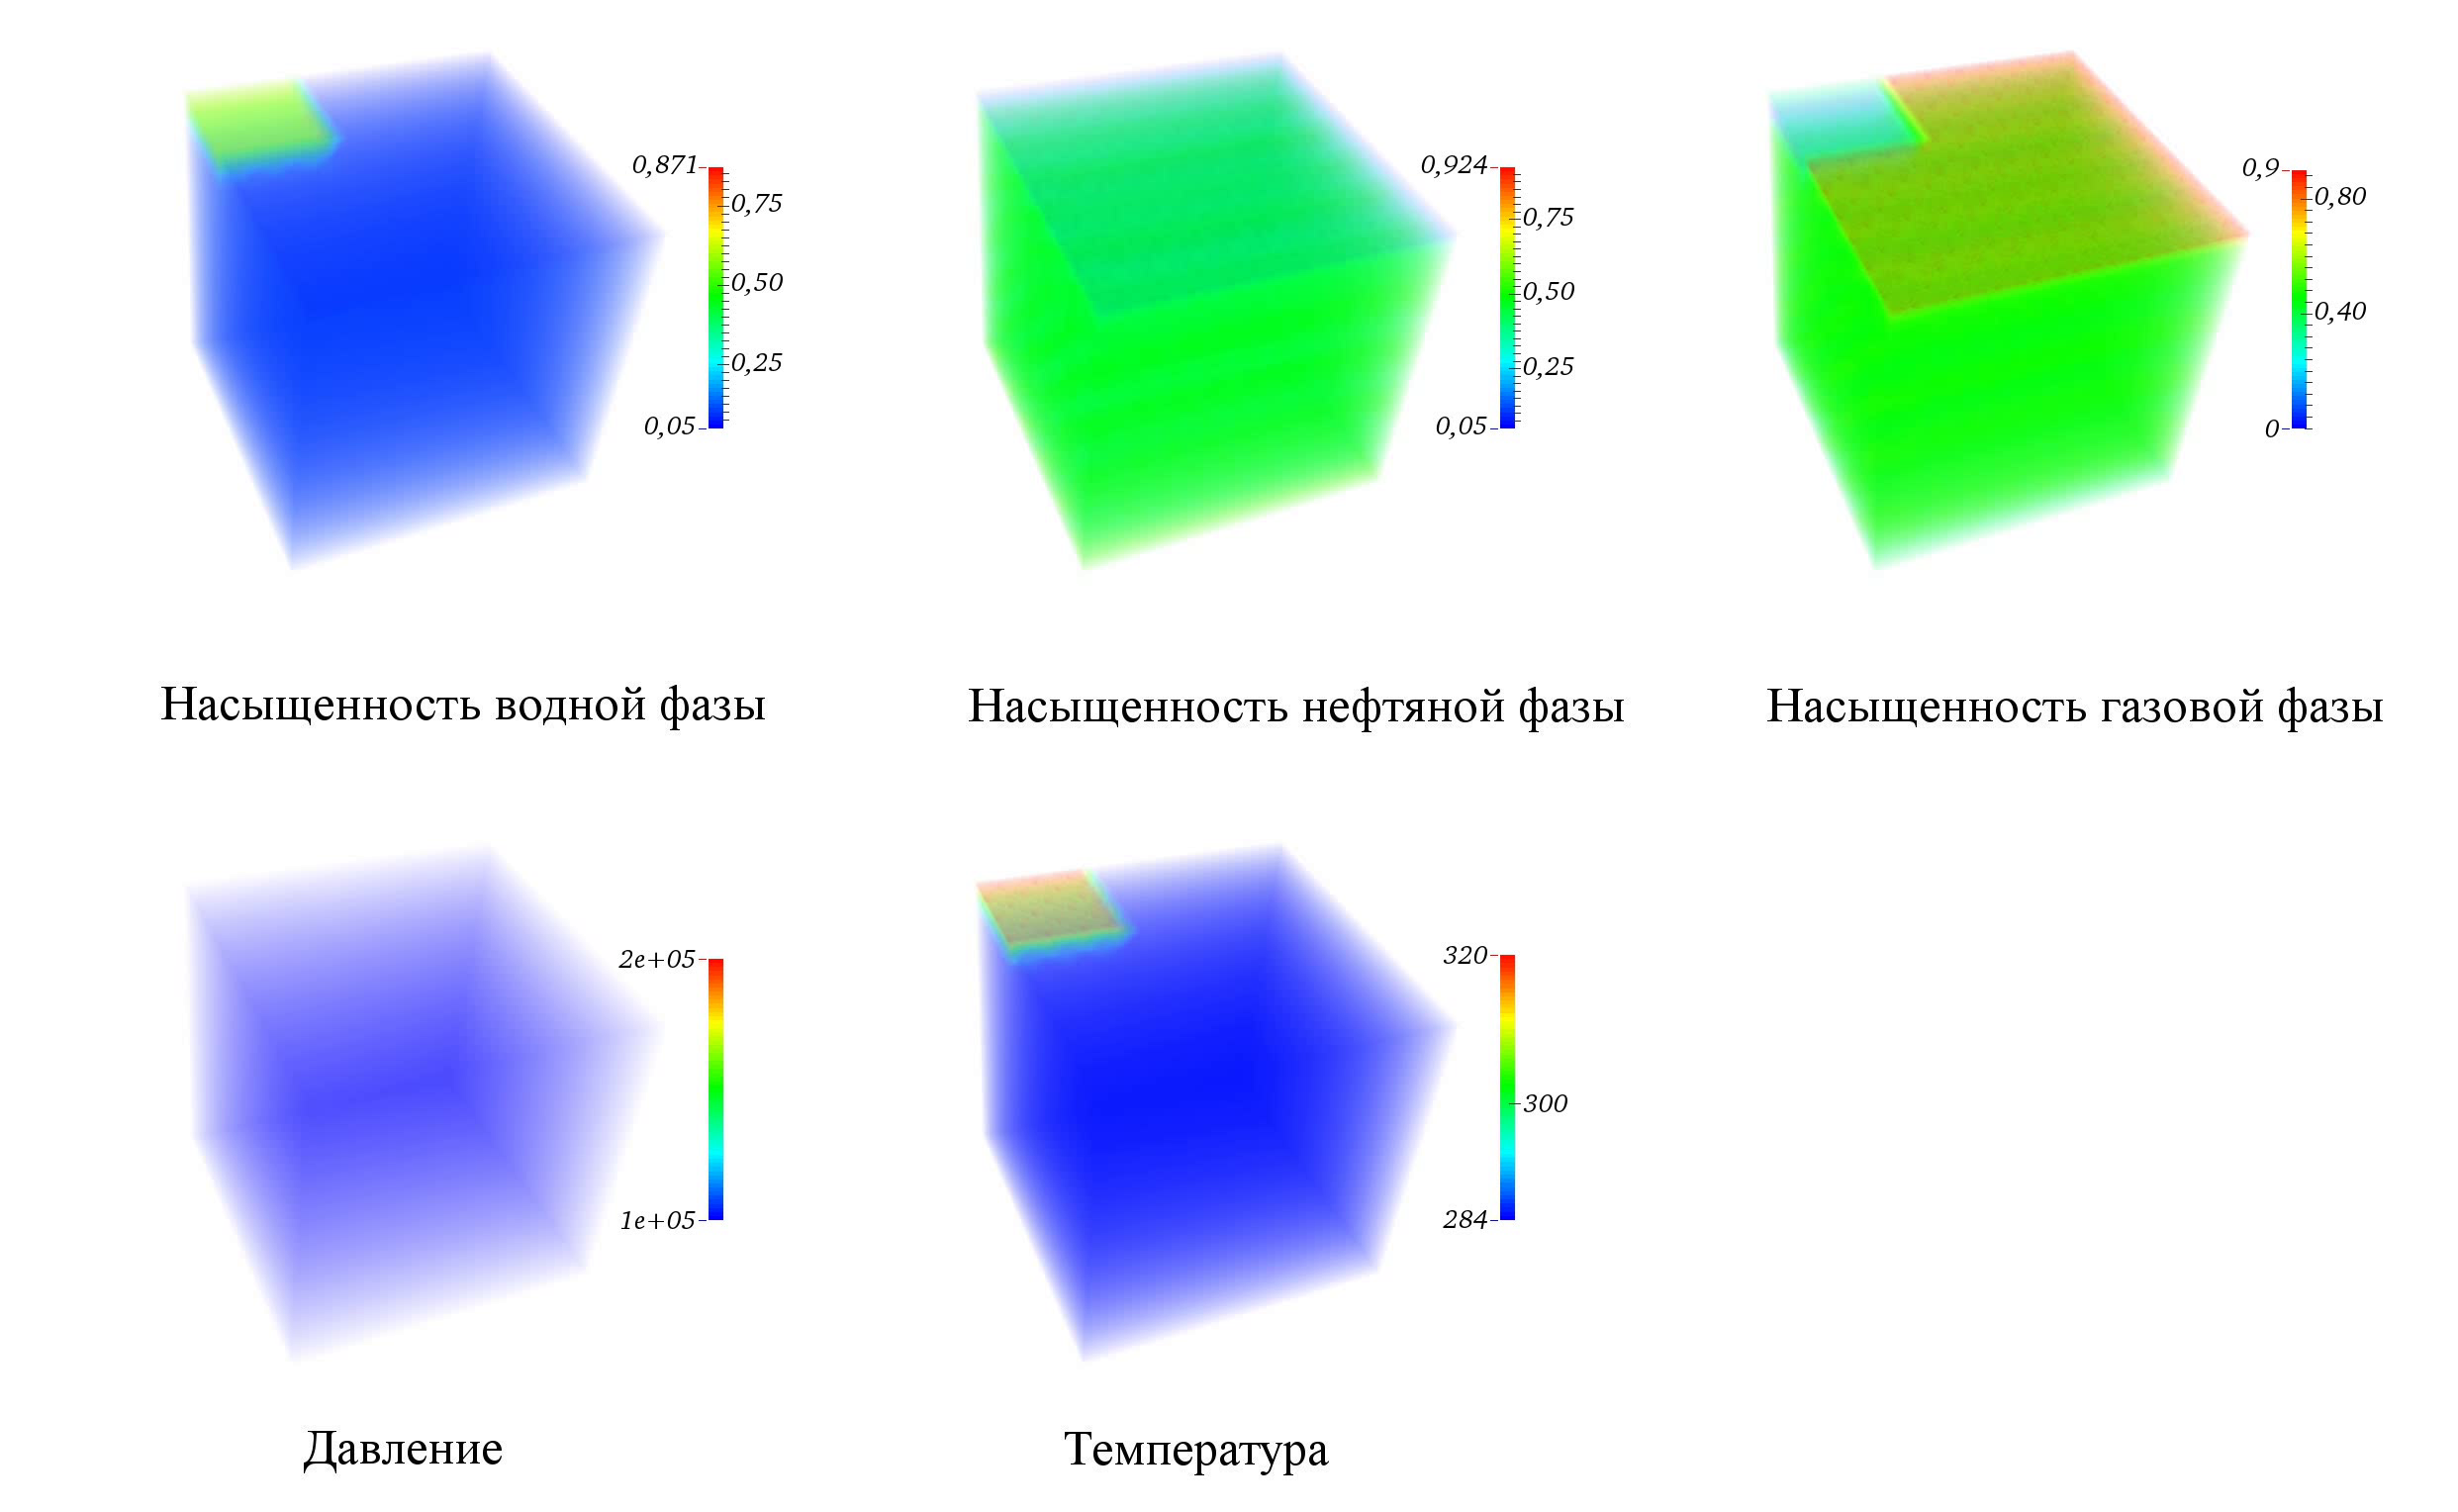
\includegraphics[width=1.0\textwidth]{video/frame.png}}{video/all_full.avi}
\end{figure}
  \end{center}
\end{frame}


\section{Анализ производительности вычислений}

\begin{frame}
\begin{center}
\frametitle{Анализ производительности вычислений}
\framesubtitle{Многопроцессорная система}
\begin{figure}[!h]
\begin{minipage}[h]{0.46\textwidth}
\begin{tikzpicture}
  \begin{axis}[axis lines=left, enlargelimits=true, grid=major, width=1.0\textwidth, height=0.7\textheight, xlabel={\textit{число процессоров}}, ylabel={\textit{ускорение}}]
    \pgfplotstableread{data/mpi_times.txt}{\mytable}
    \pgfplotstablegetelem{0}{Y}\of{\mytable}
    \pgfmathsetmacro{\ay}{\pgfplotsretval}
    \addplot [blue, mark=*] table [x=X, y expr=\ay/\thisrow{Y}] {\mytable};
  \end{axis}
\end{tikzpicture}
%\caption{Зависимость ускорения расчета тестовой задачи от числа процессоров}
\label{mpi_speedup}
\end{minipage}
\hfill
\begin{minipage}[h]{0.46\textwidth}
\begin{tikzpicture}
  \begin{axis}[axis lines=left, enlargelimits=true, grid=major, width=1.0\textwidth, height=0.7\textheight, xlabel={\textit{число процессоров}}, ylabel={\textit{эффективность}}]
    \pgfplotstableread{data/mpi_times.txt}{\mytable}
    \pgfplotstablegetelem{0}{Y}\of{\mytable}
    \pgfmathsetmacro{\ay}{\pgfplotsretval}
    \addplot [blue,mark=*] table [x=X, y expr=\ay/\thisrow{Y}/\thisrow{X}] {\mytable};
  \end{axis}
\end{tikzpicture}
%\caption{Зависимость эффективности расчета тестовой задачи от числа процессоров}
\label{mpi_eff}
\end{minipage}
\end{figure}
\end{center}
\end{frame}

\begin{frame}
\begin{center}
\frametitle{Анализ производительности вычислений}
\framesubtitle{Графический ускоритель}
\begin{figure}[!h]
\begin{center}
\begin{tikzpicture}
  \begin{axis}[axis lines=left, enlargelimits=true, grid=major, width=0.6\textwidth, xlabel={\textit{число узлов сетки}}, ylabel={\textit{ускорение}}]
    \pgfplotstableread[skip first n=1]{data/cpu_vs_gpu.txt}{\mytable}
    \addplot [blue, mark=*] table [x=0, y expr=\thisrow{1}/\thisrow{2}] {\mytable};
  \end{axis}
\end{tikzpicture}
\caption{GPU vs CPU}
\label{cuda_speedup}
\end{center}
\end{figure}
\end{center}
\end{frame}

\section{Заключение}
\begin{frame}
\begin{center}
\frametitle{Заключение}
\framesubtitle{\ }
В процессе работы над дипломом:
\begin{itemize}
  \item предложены 1D, 2D и 3D-модели трехфазных течений в пористых средах;
  \item разработан алгоритм расчета;
  \item алгоритм расчета распараллелен;
  \item написан программный комплекс;
  \item в необходимом объеме освоены технологии MPI, Nvidia CUDA, визуализации данных расчетов;
  \item программный комплекс протестирован на нескольких тестовых задачах 
  фильтрации;
  \item сделаны три доклада на конференциях, одна из которых -- международная;
  \item написаны в соавторстве две статьи.
\end{itemize}
\end{center}
\end{frame}

\begin{frame}
\begin{center}
\frametitle{\ }
\framesubtitle{\ }
\item {\huge Спасибо за внимание!}
\end{center}
\end{frame}

\end{document}
